In der Abbildung \ref{fig:Aufbau} ist der schematische Aufbau der Aperatur zu sehen.
Das G.M.-Zählrohr ist zusetzlich noch mit einem elektrischen Zählwerk verbunden.
Als erstes wird eine Nullmessung über \SI{900}{s} durchgeführt damit die Hintergrundstrahlung bestimmt werden kann.\\

Es wird ein $\gamma$-Strahler (\SI{137}{Cs}) in Halterung eingesetzt und für 8 verschiedene Dicken von Blei und Eisen die Aktivität gemessen.
Die Messzeit wird dabei so gewählt, dass der statistische Fehler ($\sigma=\frac{\sqrt{N}}{N}$) ca. bei 0,05 liegt.

Nun wird ein $\beta$-Strahler (\SI{99}{Tc}) in die Apperatur eingesetzt und für 11 verschieden dicke Aluminiumplatten die Aktivität gemessen.
Die Messzeit wird wieder dem statistischen Fehler angepasst.
\begin{figure}[h!]
  \centering
  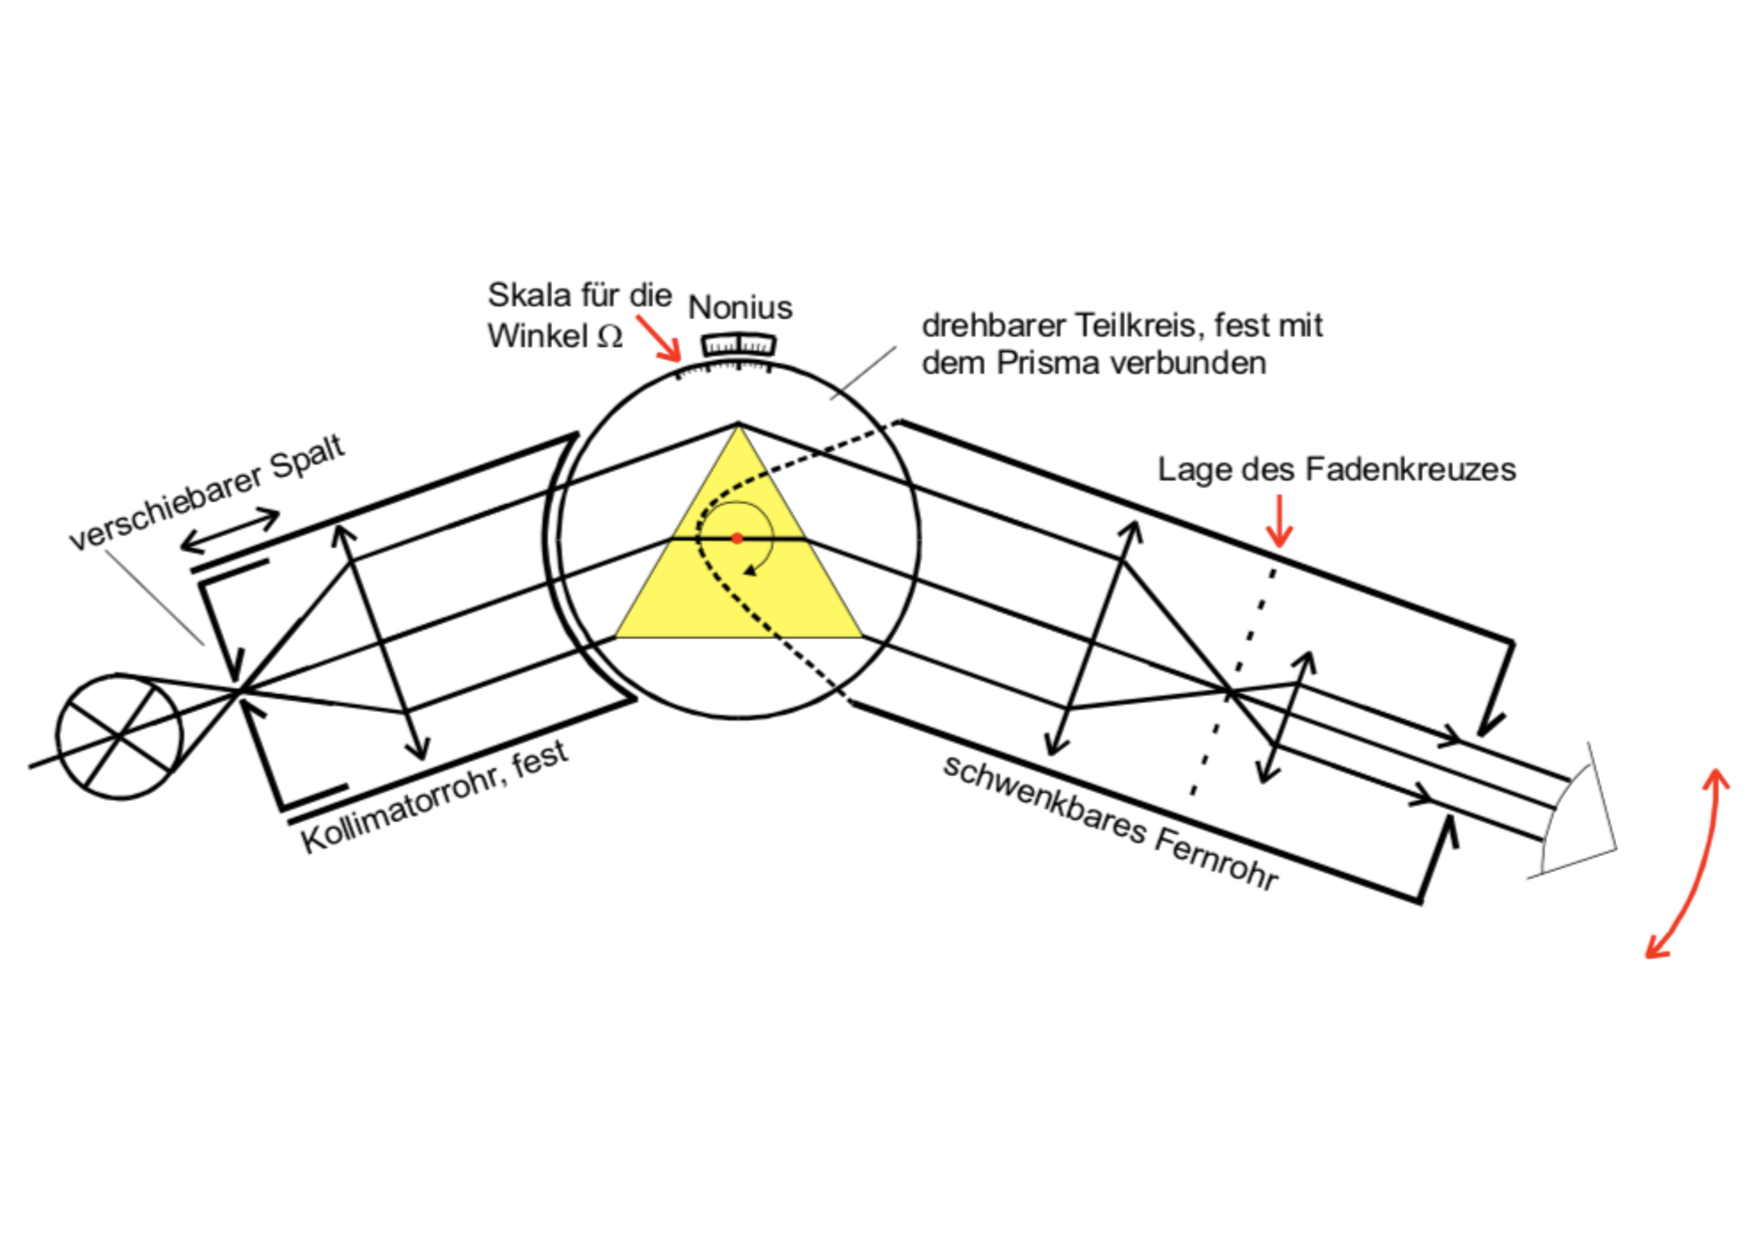
\includegraphics[width=\textwidth]{aufbau.pdf}
  \caption{Aufbau der Messapparatur \cite{1}}
  \label{fig:Aufbau}
\end{figure}
